\documentclass[prb,twocolumn,superscriptaddress,floatfix,10pt]{revtex4-2}
\usepackage{amsmath,amssymb,bm}
\usepackage{graphicx}
\usepackage[dvipsnames]{xcolor}
\usepackage[colorlinks=true,linkcolor=blue!50!black,citecolor=blue!50!black,urlcolor=blue!50!black]{hyperref}

\newcommand{\Cf}{C_{\rm eff}}
\newcommand{\Creg}{C_{\rm reg}}
\newcommand{\Qh}{Q_{\rm hole}}
\newcommand{\Ac}{A_c}
\newcommand{\dd}{\mathrm{d}}

\begin{document}

\title{Lensing of moir\'e patterns by atomic area defects:\\ topological node charge, dressed charge, and the ring-traction identity}

\author{Changyeon Won}
\email{cywon@khu.ac.kr}
\affiliation{Department of Physics, Kyung Hee University, Seoul 02447, Republic of Korea}

\date{\today}

\begin{abstract}
A point defect in one layer of a bilayer---a vacancy cluster, an inserted patch, or a locally rotated region---bends the moir\'e domain-wall network over distances far larger than the defect itself and can make moir\'e nodes disappear. We ask how many nodes an atomic defect removes, where they go, and what controls the answer. Treating the moir\'e pattern as the registry map $u:\Sigma\to T^2$, AA nodes are its degree density and obey an exact Gauss law in which every hole carries an integer charge. An atomic defect with area deficit and torque combined into a complex charge $C$ acts on the moir\'e level as a point-mass gravitational lens $\beta=z-m/\bar z$ with mass $m=C/\kappa$, where $\kappa=\theta e^{i\alpha}$ encodes twist or lattice mismatch. The lens geometry splits the removed node charge $2\pi\theta|C|/A_c$ exactly into a far share $\cos\varphi_m$ and a locally bound integer share $1-\cos\varphi_m$, with $\varphi_m=\arg C-\alpha$. Relaxed continuum simulations confirm the Gauss law without error and the local integers in seven of eight defect types, and show that the far charge is set by a \emph{dressed} charge $C_{\rm eff}=\sum C+C_{\rm reg}$. The induced part $C_{\rm reg}$ is the force dipole of the registry forces, depends on which integer branch the pattern selects, and is nearly independent of the elastic bulk modulus. We also measure the elastic constants of the moir\'e crystal itself: the twisted moir\'e has a negative bulk modulus and the mismatch moir\'e a negative rotational stiffness. Nevertheless, a ring-traction identity shows that local sources couple to the atomic traction on their boundary, not to these moir\'e constants, so no universal moir\'e response coefficient exists. The results give a counting rule for moir\'e nodes around atomic-scale damage that can be tested by scanning-probe imaging.
\end{abstract}

\maketitle

%=====================================================================
\section{Introduction}
%=====================================================================

Two lattices stacked with a small twist angle or a small lattice mismatch form a moir\'e superlattice whose period exceeds the atomic spacing by a factor $1/\theta$. Since the discovery of correlated and superconducting phases in magic-angle graphene~\cite{Bistritzer2011,Cao2018a,Cao2018b}, moir\'e systems have become a platform for engineering band structures and interactions~\cite{Andrei2020,Kennes2021}. The relevant length scale is set by the \emph{relaxed} moir\'e pattern: interlayer adhesion turns the smooth interference pattern into AB/BA domains separated by shear solitons that meet at AA nodes~\cite{Popov2011,Alden2013,Nam2017,Carr2018,Yoo2019,Dai2016,Gargiulo2018,Zhang2018}. Because the moir\'e magnifies the relative displacement of the two layers by $1/\theta$, it is extremely sensitive to strain. Twist-angle disorder, heterostrain, and local strain fields are visible directly in scanning-probe and diffraction maps~\cite{Uri2020,Kerelsky2019,Huder2018,Kazmierczak2021,Halbertal2021,Lau2022}.

Point defects are an equally natural source of local strain. Vacancy clusters, ion-irradiation craters, adatom patches and grain-boundary fragments are common in two-dimensional crystals~\cite{Banhart2011}. A cluster of a few tens of missing atoms produces a long-ranged displacement field of order $|C|/r$. In the moir\'e pattern this field is amplified by $1/\theta$ into a distortion comparable to the moir\'e period. Two questions then arise: \emph{how many moir\'e nodes does an atomic defect remove, and where does that missing node charge reside?} The answer is not obvious. The number of missing atoms is an integer, the number of moir\'e nodes is an integer, and yet the conversion factor between them is the continuous parameter $\theta$.

In this paper we answer these questions within a minimal continuum model. Four results stand out.

(i) \emph{Moir\'e nodes are topological charges.} The moir\'e pattern is a map $u$ from the sample to the registry torus $T^2$. AA nodes are the points where $u$ takes the AA value, counted with the sign of $\det\nabla u$; they are the degree density of $u$. A Gauss law fixes the node count in any region from boundary data alone, and every hole carries an integer charge.

(ii) \emph{An atomic area defect is a gravitational lens for the moir\'e.} The far field $-C/\bar z$ of a defect with complex charge $C$ (area deficit plus torque) maps the undeformed moir\'e coordinate $\beta$ to the physical coordinate $z$ through $\beta=z-m/\bar z$, the point-mass lens equation~\cite{Einstein1936,Schneider1992}, with lens mass $m=C/\kappa$. Undeformed moir\'e nodes play the role of light sources. Sources inside a disk of radius $b_s=2R|\sin(\varphi_m/2)|$ have no images and are swallowed by the defect. As a result, the removed node charge $2\pi\theta|C|/A_c$ splits into a far share $\propto\cos\varphi_m$ and a local share $\propto 1-\cos\varphi_m$, both fixed by the single phase $\varphi_m=\arg C-\alpha$.

(iii) \emph{The far charge is dressed by the moir\'e.} The registry forces redistribute when the defect reorganizes the wall network, and their force dipole adds an induced charge $C_{\rm reg}$. The far node charge is fixed by $C_{\rm eff}=\sum C+C_{\rm reg}$, not by the atomic charge alone. $C_{\rm reg}$ depends on the integer branch selected by the pattern, and it behaves as a displacement-controlled rather than a force-controlled source.

(iv) \emph{There is no universal moir\'e response coefficient.} We measure the elastic constants of the moir\'e crystal. The twisted moir\'e has a negative bulk modulus $K_M<0$, the mismatch moir\'e a negative rotational stiffness $\chi_M<0$. One might expect the far response to any local moir\'e-scale source to follow from these constants. An exact ring-traction identity shows instead that local sources couple only to the \emph{atomic} traction on their boundary. Consequently the far field is not fixed by $K_M$ and $\mu_M$, and integer bookkeeping plus the force-dipole dressing is the complete description.

Figure~\ref{fig:concept} summarizes the central picture. Section~\ref{sec:model} introduces the model, Sec.~\ref{sec:topo} the topology of the registry map, and Sec.~\ref{sec:lens} the lens map and the partition theorem. Section~\ref{sec:many} treats several defects and the conservation of far charge. Section~\ref{sec:dressed} introduces the dressed charge. Section~\ref{sec:elastic} discusses moir\'e elasticity and the ring-traction identity, and Sec.~\ref{sec:disc} discusses experimental consequences.

\begin{figure*}[t]
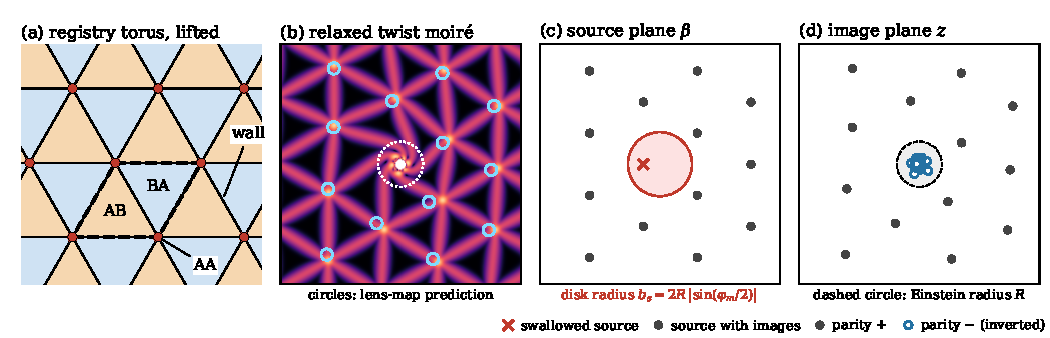
\includegraphics[width=\textwidth]{figs/fig1.pdf}
\caption{Moir\'e nodes as lensed images.
(a) Universal cover of the registry torus $T^2=\mathbb{R}^2/\Lambda$. The three line families $\mathcal{L}$ are the domain walls, the up (down) triangles are AB (BA) stacking, and the lattice points are AA. The dashed parallelogram is one fundamental cell.
(b) Relaxed twisted moir\'e ($\theta=1/30$) around an area-removing defect ($C=4$, white disk); color shows the registry energy $V(u)$. Circles mark the positive-parity images predicted by the lens map; the dotted circle is the Einstein radius $R=\sqrt{|C|/\theta}$.
(c) Source plane $\beta$: undeformed node positions. Sources inside the disk of radius $b_s$ (crosses) have no images.
(d) Image plane $z$ for the same lens ($\varphi_m=-90^\circ$). Each surviving source has an ordinary image outside $R$ (filled) and an inverted image inside $R$ (open).}
\label{fig:concept}
\end{figure*}

%=====================================================================
\section{Model}\label{sec:model}
%=====================================================================

The dynamical variable is the interlayer relative displacement $u(\bm r)\in\mathbb{R}^2$; we use complex notation $z=x+iy$, $u=u_x+iu_y$. The energy is
\begin{equation}
E[u]=\int_\Sigma\Big[\mu\,\varepsilon_{ij}\varepsilon_{ij}+\frac{\lambda}{2}\varepsilon_{kk}^2+V(u)\Big]\dd^2r,
\label{eq:E}
\end{equation}
with $\varepsilon=\tfrac12(\nabla\delta u+\nabla\delta u^{T})$ and $\delta u=u-u_b$. The background $u_b=c_{\rm AA}+\kappa z$ with $\kappa=\theta e^{i\alpha}$ describes a twist ($\alpha=90^\circ$) or an isotropic lattice mismatch ($\alpha=0$).

The registry potential is
\begin{equation}
V(u)=V_0\sum_{\bm G}\big(1-\cos\bm G\cdot u\big)+V_3\sum_{\bm G}\sin\bm G\cdot u ,
\end{equation}
where $\bm G$ runs over three reciprocal vectors of the triangular lattice $\Lambda$ (lattice constant $a=1$, cell area $A_c=\sqrt3/2$) and $V_3=\sqrt3V_0$. This honeycomb-type registry has a maximum at AA and degenerate minima at AB and BA. It is $C_6$ symmetric about AA, including layer exchange $u\to-u$, and has a mirror symmetry~\cite{Popov2011,Nam2017}.

\emph{Iris defects.} A defect at $z_k$ is a disk of radius $r_h$ removed from the energy. A penalty fixes the mean normal and tangential displacement of its rim, $\langle\delta u\cdot n\rangle=-{\rm Re}\,C/r_h$ and $\langle\delta u\cdot t\rangle=-{\rm Im}\,C/r_h$, while the rim shape is free. The complex charge $C=|C|e^{i\psi}$ combines an area deficit ($C>0$, a ``closed iris''), an inserted area ($C<0$), and a rim rotation or point torque (${\rm Im}\,C\ne0$). In an infinite medium the equilibrium field is
\begin{equation}
\delta u=-\frac{C}{\bar z-\bar z_k}.
\label{eq:lensfield}
\end{equation}
It is the gradient of a harmonic potential, so ${\rm div}\,\delta u={\rm curl}\,\delta u=0$ and it solves Eq.~\eqref{eq:E} for any $\lambda,\mu$ (pure shear). A defect that removes $n_{\rm miss}$ unit cells has $C=n_{\rm miss}A_c/2\pi$, as measured by the displacement flux far away.

\emph{Numerics.} We minimize Eq.~\eqref{eq:E} with L-BFGS~\cite{Liu1989} on a square grid of spacing $h=0.45$ with $u=u_b$ on the outer boundary. The standard box has half-width $72$; the large boxes have half-width $148.5$ (grid $661^2$, about 105 nodes). Unless noted, $\theta=1/30$, $V_0=0.005$, $\mu=1$, $\lambda=-0.5$ (2D bulk modulus $K=\lambda+\mu$, $K/\mu=0.5$), $|C|=4$, $r_h=2.4$. The lens (Einstein) radius is $R=\sqrt{|C|/\theta}\approx11$ and the relaxed moir\'e period is $\approx31$. All parameters are collected in Table~\ref{tab:param} (Appendix~\ref{app:num}).

%=====================================================================
\section{Topology of the registry map}\label{sec:topo}
%=====================================================================

\subsection{Degree and the wall network}

An affine registry $u=c+Az$ ($\det A\ne0$) maps the moir\'e lattice $\Lambda_M=A^{-1}\Lambda$ onto $\Lambda$. It therefore induces a homeomorphism $\mathbb{R}^2/\Lambda_M\to T^2$ of degree ${\rm sign}\det A$; in complex notation $u=\kappa z+\eta\bar z$ gives $\det A=|\kappa|^2-|\eta|^2$. Twist and isotropic mismatch have degree $+1$; a strain dominated by $\bar z$ has degree $-1$.

Cutting $T^2$ into AB and BA regions gives its minimal triangulation: one vertex (AA), three edges, and two faces, with Euler number zero [Fig.~\ref{fig:concept}(a)]. In the universal cover $\mathbb{R}^2$ the one-skeleton is the arrangement $\mathcal L$ of three families of lines through the AA lattice points. We define the domain walls as $u^{-1}(\mathcal L)$ and the nodes as $u^{-1}({\rm AA}+\Lambda)$. Two consequences follow:

\emph{Even valence.} Any generic closed loop crosses each line of $\mathcal L$ an even number of times, because the AB/BA faces alternate (a two-coloring). Hence the number $z$ of walls meeting at a vertex, or crossed by a loop around a defect core, is even. Ordinary AA nodes have $z=6$; the eight- and ten-wall vertices seen near defects obey the same rule. Where all faces are triangles, Euler's theorem gives $\sum_v(6-z_v)=6\chi$, so a core behaves like a vertex carrying disclination charge $6-z_{\rm core}$~\cite{Nelson2002,Kleman2008}.

\subsection{Node charge and Gauss law}

A loop $\gamma$ with vanishing Burgers class $\oint_\gamma\dd u\in\Lambda$ lifts to $\mathbb{R}^2$; iris defects have zero Burgers class. We define the node charge
\begin{equation}
Q(\gamma)=\sum_{n\in\Lambda}{\rm wind}\big(\tilde u\circ\gamma,\;c_{\rm AA}+n\big)\in\mathbb{Z},
\end{equation}
which is invariant under deformations that do not cross a node. At a regular point the index of a node is ${\rm sign}\det\nabla u=\pm1$: ordinary nodes $N_+$ and inverted nodes $N_-$. For a region $D$ containing holes $H_k$ (defect cores) on whose complement $u$ is continuous,
\begin{equation}
N_+(D)-N_-(D)+\sum_k Q(\partial H_k)=Q(\partial D),
\label{eq:gauss}
\end{equation}
with node density $\rho_N=\det\nabla u/A_c$.
The proof uses additivity of winding numbers: interior edges of a fine subdivision cancel, and a cell containing one node contributes its local degree. Because $\rho_N$ is a null Lagrangian, $\partial_t\rho_N+\nabla\cdot j=0$ holds identically in any continuous dynamics. Nodes therefore enter or leave only through holes, or are created and annihilated in $\pm$ pairs~\cite{Mermin1979}. This is the sense in which moir\'e nodes are conserved charges.

\emph{Valence--winding bound.} If the AA points enclosed by the lift of $\gamma$ have windings $0$ or $\pm1$ of one sign with total $w$, then
\begin{equation}
z(\gamma)\ge 2L_{\min}(|w|),\qquad z(\gamma)\in2\mathbb{Z},
\label{eq:zw}
\end{equation}
where $L_{\min}(n)$ is the minimum number of lattice lines of the three families needed to cover $n$ triangular-lattice points ($L_{\min}=3,5,6,7,8,9,9$ for $n=1,\dots,7$). By a Jordan-curve argument, each line through an enclosed point is crossed at least twice. The bound is $2L_{\min}$ rather than $6|w|$ because neighboring points share lines.

\emph{Numerical checks.} The discrete count used throughout (Appendix~\ref{app:count}) makes Eq.~\eqref{eq:gauss} exact on the grid. Over 84 relaxed states (backgrounds, single defects, and every branch of the pairs) the Gauss law holds with zero deviation [Fig.~\ref{fig:topo}(a)]. A single area-removing defect in the twisted moir\'e has $Q_{\rm hole}=5$ and $N_-=4$, so it binds $q\equiv Q_{\rm hole}-N_-=+1$ node; in the mismatch moir\'e $Q_{\rm hole}=N_-=2$, so $q=0$ [Fig.~\ref{fig:topo}(b)]. Among 444 circles around cores, Eq.~\eqref{eq:zw} is never violated and 162 circles saturate it [Fig.~\ref{fig:topo}(c)].

\begin{figure*}[t]
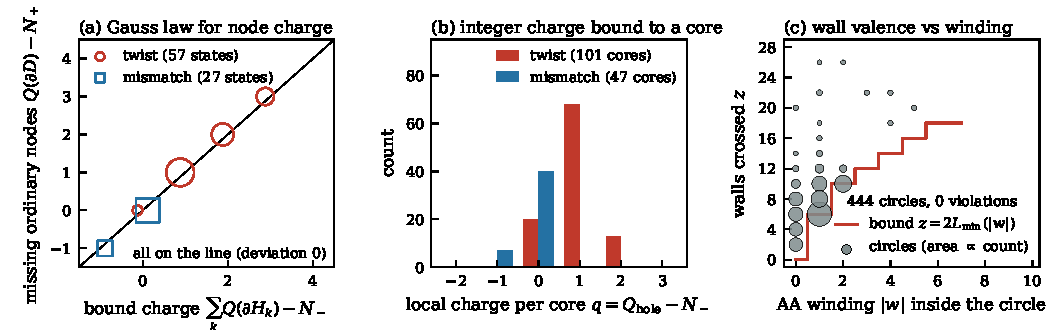
\includegraphics[width=\textwidth]{figs/fig2.pdf}
\caption{Topological charges of the registry map.
(a) Gauss law, Eq.~\eqref{eq:gauss}: the ordinary-node deficit equals the charge bound to holes and inverted nodes in all 84 states. Symbol area is proportional to the number of states.
(b) Distribution of the integer charge $q=Q_{\rm hole}-N_-$ bound to a single core, over all single-defect and pair states ($K/\mu=0.5$).
(c) Number of walls $z$ crossed by circles of radius 5, 7, 9 around cores versus the AA winding $|w|$ they enclose. The red staircase is the bound of Eq.~\eqref{eq:zw}.}
\label{fig:topo}
\end{figure*}

%=====================================================================
\section{Area defects as gravitational lenses}\label{sec:lens}
%=====================================================================

\subsection{Complex charge}

For any loop around a set of defects, Eq.~\eqref{eq:lensfield} gives
\begin{equation}
\oint_\gamma\delta u\cdot(n+i\,t)\,\dd s=-2\pi\sum_k C_k .
\end{equation}
Thus $C$ is a conserved charge, and $C$ and $-C$ can be created or annihilated in pairs. However, the field~\eqref{eq:lensfield} is traceless and curl-free, so it does no first-order work on a dilatation or torque center. Two such charges therefore have no long-range elastic interaction regardless of their signs, as for Eshelby inclusions in an infinite medium~\cite{Eshelby1957}. Elasticity alone is sign-blind.

\subsection{Lens map}

Writing $u=c+\kappa\beta$ defines the undeformed moir\'e coordinate $\beta$. For one defect at the origin,
\begin{equation}
\beta(z)=z-\frac{m}{\bar z},\qquad m=\frac{C}{\kappa}=R^2e^{i\varphi_m},
\label{eq:lens}
\end{equation}
with Einstein radius $R=\sqrt{|C|/\theta}$ and mass phase $\varphi_m=\arg C-\alpha$.
This is the lens equation of a point mass, with source position $\beta$ and image position $z$~\cite{Einstein1936,Schneider1992}. The lens mass $m$ is the defect charge transferred to the moir\'e level, and the undeformed moir\'e nodes form a perfect lattice of density $n_M=\theta^2/A_c$ in the source plane. The Jacobian $J=1-R^4/|z|^4$ is negative inside the Einstein circle, where images are inverted.

\emph{Image structure.} Let $z=re^{i\phi}$. Then $|\beta|^2=r^2+R^4/r^2-2R^2\cos\varphi_m$. A source at $|\beta|=b$ therefore has no image if
\begin{equation}
b<b_s=2R\,\big|\sin(\varphi_m/2)\big| ,
\label{eq:bs}
\end{equation}
and otherwise has one ordinary image at $r_+>R$ and one inverted image at $r_-=R^2/r_+$. In the gravitational analogy the disk $b<b_s$ is the shadow of the lens. Its size depends on the relative phase of the defect charge and the moir\'e background. For an area defect in a twisted moir\'e, $\varphi_m=\mp90^\circ$ and $b_s=\sqrt2R$. For an area defect in a mismatch moir\'e, $\varphi_m=0$ and nothing is swallowed. Figure~\ref{fig:concept}(b) shows that the predicted ordinary images coincide with the relaxed AA nodes outside the core region.

\subsection{Partition theorem}

Averaging over random translations of the moir\'e lattice, the expected number of sources in a region $S$ of the source plane is $n_M|S|$. Positive images inside $|z|<\rho$ correspond one-to-one to sources with $b_s<b<b(\rho)=|\rho-m/\rho|$, and the loop $|z|=\rho$ maps onto a curve enclosing area $\pi b(\rho)^2$. For $\rho>R$ this yields
\begin{align}
\Delta N_+(\rho)&=T-\frac{\pi n_MR^4}{\rho^2},\qquad T\equiv\frac{2\pi\theta|C|}{A_c},\nonumber\\
\Delta Q(\rho)&=-\frac{2\pi}{A_c}{\rm Re}(\bar\kappa C)+\frac{\pi n_MR^4}{\rho^2},\nonumber\\
q&=Q_{\rm hole}-N_-=T\,(1-\cos\varphi_m),
\label{eq:partition}
\end{align}
which are tied together by the Gauss law $q=\Delta N_++\Delta Q$; here we used $n_MR^2\cos\varphi_m={\rm Re}(\bar\kappa C)/A_c$. The ordinary-node deficit at infinity, $T=\theta\,n_{\rm miss}$, is independent of $\varphi_m$: \emph{a defect missing $n_{\rm miss}$ unit cells removes $\theta n_{\rm miss}$ moir\'e nodes}. Of these, the share $T(1-\cos\varphi_m)$ is swallowed and bound to the core, and the share $T\cos\varphi_m$ is spread to infinity as boundary charge $\Delta Q$. For our parameters $T=0.967$.

In the relaxed moir\'e the local share must be an integer. Equation~\eqref{eq:partition} becomes a rounding rule, and the deviations are carried by the far share. Figure~\ref{fig:partition} and Table~\ref{tab:eight} compare the eight defects $C=\pm4,\pm4i$ in both backgrounds. In seven of the eight, the bound integer $q$ equals the rounded prediction. The exception, a torque opposing the twist ($\varphi_m=180^\circ$), binds $q=1$ instead of $2$ and is probably metastable. The far share $-\Delta Q$ follows $T\cos\varphi_m$ [open symbols in Fig.~\ref{fig:partition}(b)].

\begin{figure*}[t]
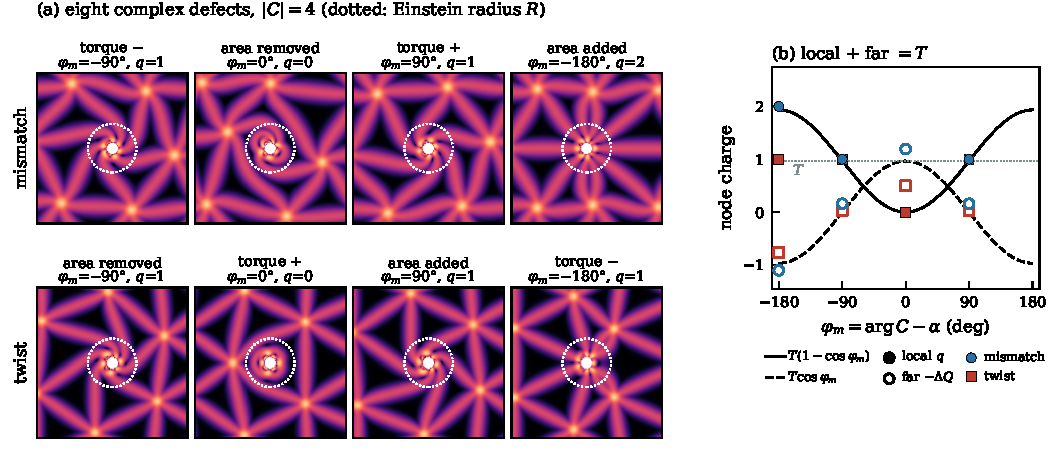
\includegraphics[width=\textwidth]{figs/fig3.pdf}
\caption{Partition of the removed node charge.
(a) Registry energy around the eight defects $C=\pm4,\pm4i$ in the mismatch (top) and twisted (bottom) moir\'e, ordered by $\varphi_m$. Each title gives $\varphi_m$ and the integer $q$ bound to the core.
(b) Local share $q$ (filled) and far share $-\Delta Q$ (open, averaged over $36<\rho<58$) versus $\varphi_m$, compared with $T(1-\cos\varphi_m)$ and $T\cos\varphi_m$, where $T=2\pi\theta|C|/A_c=0.967$. Blue circles: mismatch; red squares: twist.}
\label{fig:partition}
\end{figure*}

\begin{table}[b]
\caption{Eight complex defects ($|C|=4$). Predicted local share $T(1-\cos\varphi_m)$, measured bound integer $q$, and defect energy relative to the background.}
\label{tab:eight}
\begin{ruledtabular}
\begin{tabular}{lcccc}
defect & $\varphi_m$ & pred. & $q$ & $E-E_{\rm bg}$\\
\hline
mismatch, area removed & $0^\circ$ & 0.00 & 0 & 14.34\\
mismatch, torque $\pm$ & $\pm90^\circ$ & 0.97 & 1, 1 & 14.75, 14.75\\
mismatch, area added & $180^\circ$ & 1.93 & 2 & 16.20\\
twist, torque along twist & $0^\circ$ & 0.00 & 0 & 14.69\\
twist, area removed/added & $\mp90^\circ$ & 0.97 & 1, 1 & 15.74, 15.74\\
twist, torque against twist & $180^\circ$ & 1.93 & 1 & 18.25\\
\end{tabular}
\end{ruledtabular}
\end{table}

\subsection{Symmetry}

Layer exchange ($u\to-u$, an inversion about AA) maps $(\kappa,C)\to(-\kappa,-C)$ and preserves $\varphi_m$. The mirror maps $(\kappa,C)\to(\bar\kappa,\bar C)$ and sends $\varphi_m\to-\varphi_m$. Hence (a) in the twisted moir\'e, removing and adding area ($\varphi_m=\mp90^\circ$) give identical energies and integer data; (b) in the mismatch moir\'e, removing and adding area are \emph{not} related by symmetry---they bind $0$ and $2$ nodes; (c) the two torques in the mismatch moir\'e are mirror images. All three statements hold in Table~\ref{tab:eight}. In particular, a closing iris and an opening iris carry opposite conserved charge and opposite far charge, yet the same sign of bound charge, since $1-\cos\varphi_m\ge0$.

%=====================================================================
\section{Several defects: conservation and its limits}\label{sec:many}
%=====================================================================

For a large loop $\gamma$ enclosing all defects, write $u=u_b+\delta u$ on $\gamma$. To first order in $\delta u$, the area enclosed by the image curve changes by $\theta\oint[\cos\alpha\,\delta u\cdot n+\sin\alpha\,\delta u\cdot t]\dd s$. Hence
\begin{align}
Q(\gamma)-Q_{\rm bg}(\gamma)&=-\frac{2\pi}{A_c}{\rm Re}\big(\bar\kappa\,C_{\rm eff}(\gamma)\big),\label{eq:ceff}\\
C_{\rm eff}(\gamma)&=-\frac{1}{2\pi}\oint_\gamma\delta u\cdot(n+i\,t)\,\dd s ,\nonumber
\end{align}
up to terms of order $|m|^2/\rho^2$. Multipoles $e^{-in\phi}$ with $n\ge2$ do not change the area. If $\gamma$ lies in the linear region and the moir\'e induced no forces, $C_{\rm eff}=\sum_kC_k$, and the far node charge would be linear in, additive in, and conserved with the atomic charge.

Figure~\ref{fig:pairs}(a,b) tests this on single defects and pairs in the standard box. We compare $\Delta Q(\rho)$ averaged over $36<\rho<58$ with the linear prediction from $\sum C$, including the image fields of the clamped box. Over 17 states the slope is $0.81$ and the correlation $0.91$. The integer $\Delta Q(\rho)$ jumps by $\pm2$ to $\pm6$ whenever a symmetric shell of nodes crosses the loop, so individual values carry an uncertainty of about $\pm0.5$.

\emph{Pairs.} With $V_0=0$ (pure elasticity), $(+,-)$ and $(+,+)$ pairs have almost the same interaction energy: $-2.99$ and $-3.14$ at $d=8$, $+0.06$ and $-0.07$ at $d=40$ [Fig.~\ref{fig:pairs}(c)]. The moir\'e distinguishes signs only at contact. In the mismatch moir\'e at $d=0.73R$ the moir\'e-mediated energies are $U_{+-}=-1.13$ and $U_{++}=+1.03$, and the $(+,-)$ pair binds no node. Within the lens map the removed node charge is $n_M\int\min(1,|f'|^2)\dd^2z$ with $f'=-\sum_km_k/(\bar z-\bar z_k)^2$ (Appendix~\ref{app:pair}). It is subadditive for opposite charges because $|C_1+C_2|<|C_1|+|C_2|$: the attraction between a closing and an opening iris is a contact interaction of range $\sim2R$.

In the twisted moir\'e, $(+,+)$ pairs show several integer branches at the same separation, binding 1, 2, or 3 nodes in total [Fig.~\ref{fig:pairs}(d)]. Pulling the cores apart from short distance keeps a ``charge-starved'' branch (cores bind $(+1,0)$). In it, a doubled wall tethers the two cores and traps an AA node that neither core absorbs [Fig.~\ref{fig:pairs}(e)]. Pushing them together from large distance keeps the branch in which each core binds one node [Fig.~\ref{fig:pairs}(f)]. At $d=40$ the two branches differ by $4.3$ in energy. Snapping of the tether is the event in which the second core absorbs the trapped node ($q:0\to+1$). The twisted-moir\'e pair energies hardly change between $K/\mu=0.5$ and $2$: the ratio of dilational to shear strain in the twisted background is $3\times10^{-4}$, so the problem stays in the shear sector.

\begin{figure*}[t]
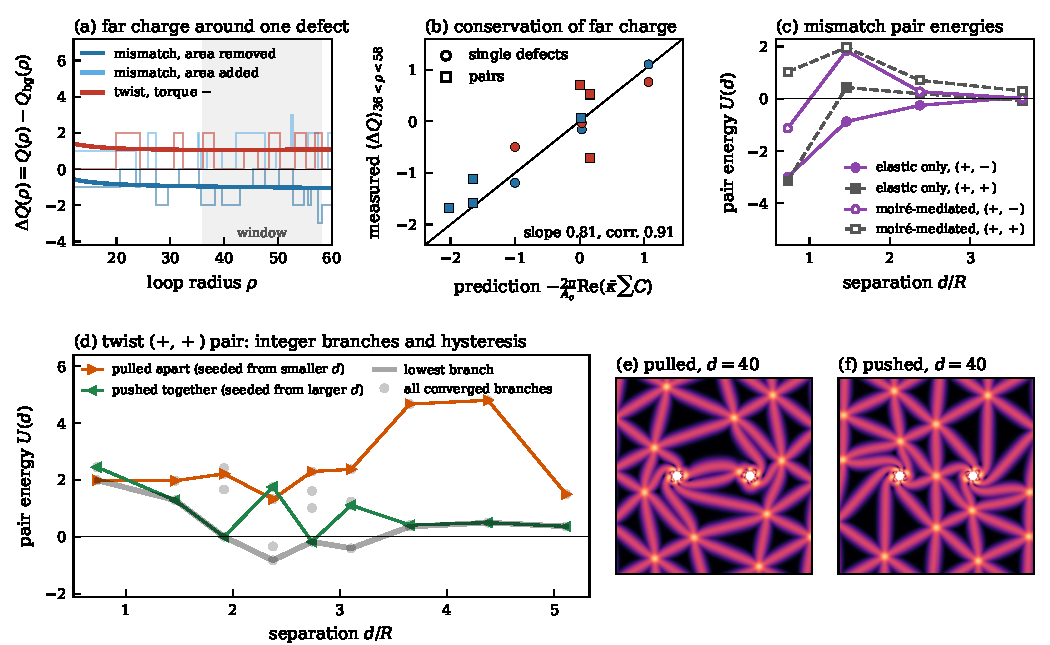
\includegraphics[width=\textwidth]{figs/fig4.pdf}
\caption{Far charge and pair interactions.
(a) Loop charge $\Delta Q(\rho)$ around single defects: integer data (thin steps) and linear prediction from $\sum C$ with box images (thick). The shaded window is used for averaging.
(b) Measured versus predicted far charge for 8 single defects (circles) and 9 pair states (squares); blue: mismatch, red: twist.
(c) Pair energy in the mismatch background: purely elastic part ($V_0=0$, filled) and moir\'e-mediated part (open) for closing--opening $(+,-)$ and closing--closing $(+,+)$ pairs.
(d) Twisted $(+,+)$ pair: energies of all converged branches (gray), of the branch followed when pulling the cores apart (orange) and pushing them together (green), and the lowest branch.
(e),(f) Local rotation $\omega=\tfrac12{\rm curl}\,u$ of the pulled and pushed states at $d=40$; walls appear as ridges. In (e) a doubled wall tethers the two cores.}
\label{fig:pairs}
\end{figure*}

%=====================================================================
\section{The dressed charge}\label{sec:dressed}
%=====================================================================

\subsection{Branches with equal atomic charge have different far charge}

To separate the far field from the box boundary we embedded the small-box branches into boxes of half-width 148.5 and relaxed them again. Two branches with the same $\sum C$ have loop charges that differ out to $\rho\approx140$ and disagree with the bare-charge prediction. Equation~\eqref{eq:ceff}, however, evaluated with the measured $C_{\rm eff}(\rho)$, reproduces the loop charge within $0.1$--$0.2$ for $\rho\ge50$ in all four states. For $\rho\gtrsim50$, $C_{\rm eff}(\rho)$ is fitted by a point source screened by the clamped edge, $C_0(1-\rho^2/L^2)$ with $L\approx152$--$166$ [Fig.~\ref{fig:dressed}(a,b)]. The reorganization of the wall network is thus confined within $\sim50$ of the pair, and farther out it appears only as a monopole $C_0\neq\sum C$.

The difference $C_{\rm reg}=C_0-C_{\rm bare}$ is an induced charge. Here $C_{\rm bare}$ is the dressed charge of a purely elastic run with identical boundary conditions; it differs from the nominal $8$ because of the rim penalty. In the twisted moir\'e a torque charge appears even though the bare torque is zero, and its sign differs between branches. In the mismatch moir\'e the area charge differs by $3.0$ between branches (Table~\ref{tab:creg}). The far node charges of the two branches differ by 2.7 (twist) and 0.7 (mismatch). \emph{The far charge is therefore not fixed by $\sum C$; the integer branch enters through $C_{\rm reg}$.}

\subsection{Force-dipole formula}

The registry force $f=-\partial V/\partial u$ is a body force acting within the layer. When a defect reorganizes the wall network, the body force changes by $\Delta f$ relative to the background. If $\Delta f$ is localized and carries no net force, then in two-dimensional Lam\'e elasticity an isotropic force dipole $P\delta_{ij}$ produces $u_r=P/[2\pi(\lambda+2\mu)r]$ and a point torque $M$ produces $u_\theta=M/(4\pi\mu r)$~\cite{Landau1986}. The traceless symmetric part produces $e^{\pm2i\phi}$ fields that carry neither flux nor circulation. Comparing with $u_r=-{\rm Re}\,C/r$ and $u_\theta=-{\rm Im}\,C/r$ gives
\begin{equation}
C_{\rm reg}=-\frac{{\rm Tr}\,P}{4\pi(\lambda+2\mu)}-i\,\frac{M}{4\pi\mu},
\label{eq:dipole}
\end{equation}
with $P_{ij}=\int x_i\,\Delta f_j\,\dd^2x$ and $M=P_{xy}-P_{yx}$.
The moir\'e lattice itself carries a periodic force distribution that cancels cell by cell. The moments must therefore be evaluated with a window that decays smoothly over more than one moir\'e period; a sharp cutoff produces large oscillations. With windows of radii 40--100 and 50--120, Eq.~\eqref{eq:dipole} reproduces the measured twist torque within $0.3$ and the area part within $0.6$ [Fig.~\ref{fig:dressed}(c)].

\begin{table*}[t]
\caption{Dressed charge in large boxes ($K/\mu=0.5$). $q$: integers bound by the two cores; $C_0$: fitted monopole; $C_{\rm reg}=C_0-C_{\rm bare}$ measured and from Eq.~\eqref{eq:dipole}; $F$: far node charge $-(2\pi/A_c){\rm Re}(\bar\kappa C_0)$. In the mismatch case only the area part enters $F$.}
\label{tab:creg}
\begin{ruledtabular}
\begin{tabular}{lccccc}
state & $q$ & $C_0$ & $C_{\rm reg}$ & $C_{\rm reg}$ [Eq.~\eqref{eq:dipole}] & $F$\\
\hline
twist, pulled & (1,0) & $6.73+7.55i$ & $-2.98+7.55i$ & $-3.6+7.3i$ & $-1.83$\\
twist, pushed & (1,1) & $8.11-3.70i$ & $-1.60-3.70i$ & $-2.1-3.4i$ & $+0.90$\\
mism., pulled & (0,$-1$) & $7.11$ & $+0.42$ & $0.0\pm1$ & $-1.72$\\
mism., pushed & (0,0) & $4.10$ & $-2.59$ & $\approx-3.0$ & $-0.99$\\
\end{tabular}
\end{ruledtabular}
\end{table*}

\subsection{The induced charge is displacement-controlled}

Equation~\eqref{eq:dipole} weights the area part by $1/(\lambda+2\mu)$. If the registry forces were fixed, the area part of $C_{\rm reg}$ would halve when $\lambda+2\mu$ doubles. We relaxed the same twisted branches at $K/\mu=2$ ($\lambda=1$, box half-width 109.8). Equation~\eqref{eq:dipole} still holds at each stiffness, but the forces are not fixed. ${\rm Tr}\,P$ grows from 68 to 127 (pulled) and from 40 to 50 (pushed), and ${\rm Re}\,C_{\rm reg}$ changes by factors $1.07$ and $0.87$ instead of $0.5$. The torque moments $M$ are almost unchanged ($-92/-79$ and $+42/+49$), as expected for a reorganization confined to the shear sector [Fig.~\ref{fig:dressed}(d)].

The registry reorganization therefore acts as a source of prescribed \emph{displacement}---the partial Burgers vectors carried by the walls---not of prescribed force. $C_{\rm reg}$ is a geometric quantity selected by the integer branch, and the force dipole is the elastic reaction needed to produce it. In the mismatch case at $K/\mu=2$ the background develops a spontaneous chirality, which makes individual $C_{\rm eff}$ unreliable. The branch difference is still well defined: ${\rm Re}\,\Delta C_{\rm reg}=2.6$ measured versus $2.55$ from Eq.~\eqref{eq:dipole}, close to the value $3.0$ at $K/\mu=0.5$.

\begin{figure*}[t]
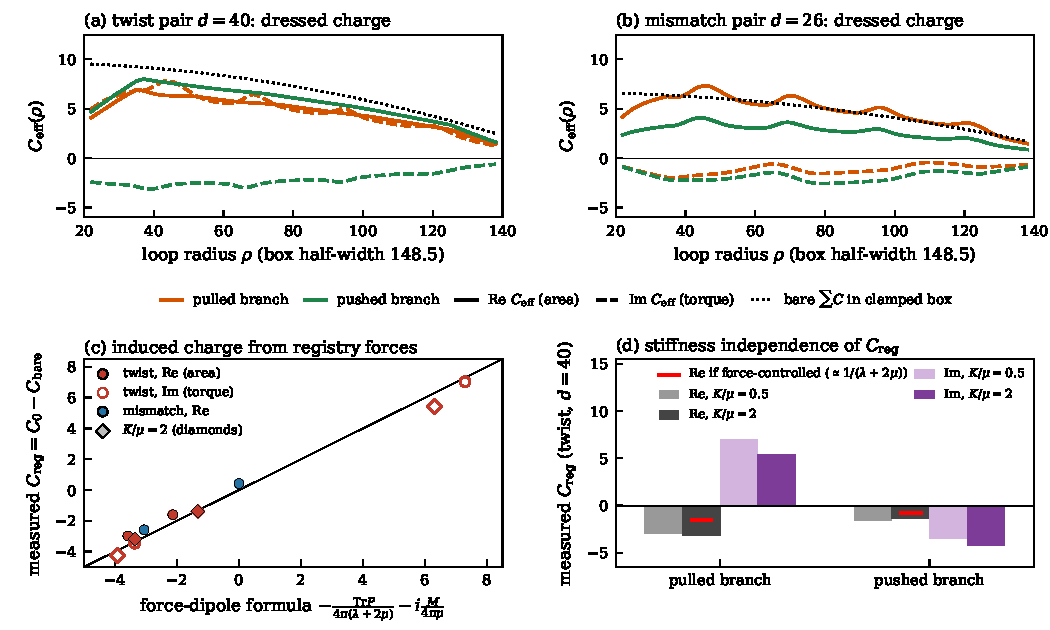
\includegraphics[width=\textwidth]{figs/fig5.pdf}
\caption{Dressed charge in large boxes (half-width 148.5).
(a),(b) Dressed charge $C_{\rm eff}(\rho)$ of the pulled and pushed branches of a twisted pair ($d=40$) and a mismatch pair ($d=26$), smoothed over one moir\'e period. Solid lines: area part; dashed lines: torque part. The dotted line is the bare charge in the clamped box.
(c) Induced charge $C_{\rm reg}$ measured versus the force-dipole formula, Eq.~\eqref{eq:dipole}, for $K/\mu=0.5$ (circles) and $K/\mu=2$ (diamonds); filled: area part, open: torque part.
(d) $C_{\rm reg}$ of the twisted pair at two stiffnesses. The red bars mark the area part expected if the registry forces were fixed ($\propto1/(\lambda+2\mu)$).}
\label{fig:dressed}
\end{figure*}

\subsection{Integer bookkeeping and moir\'e Burgers circuits}

Can $C_{\rm reg}$ be predicted from integer data? The $\kappa$-component of $C_{\rm eff}$ is exactly a node count. Consider a smooth radial window $w(r)={\rm clip}[(62-r)/32,0,1]$ and the window-weighted counts $N_{-,w}$ and $\Delta N_{+,w}$. Then
\begin{equation}
F\equiv-\frac{2\pi}{A_c}{\rm Re}(\bar\kappa C_{\rm eff})=\sum_kQ_{{\rm hole},k}-N_{-,w}-\Delta N_{+,w},
\label{eq:bookkeeping}
\end{equation}
which follows from the Gauss law. It holds within $0.07$ for all 50 pair states with $d\le40$ [Fig.~\ref{fig:book}(a)]. The bound integers $q_k$ and the core valences $z_k$ control the sign of $F$ in twisted pairs. With $\sum q=1$ and one core of valence $z\le6$, $F<0$; with $\sum q=1$ and both cores $z\ge8$, or with $\sum q\ge2$, $F>0$ [Fig.~\ref{fig:book}(b)]. The magnitude is not fixed by $(q,z)$, because the network deficit $\Delta N_{+,w}$ varies by up to one node between states with equal $(q,z)$.

The missing integer is visible in moir\'e Burgers circuits. Since $u$ is continuous, the moir\'e Burgers vector $B=A^{-1}\oint\dd u$ vanishes for every loop, so there are no true moir\'e dislocations. However, labeling every node by the AA lattice point it reaches and comparing labels with the rounded geometric steps along a Delaunay triangulation reveals geometric dislocations, i.e., 5--7-like defects of the node lattice. They occur as $\pm B$ dipoles, and only in the pulled (tethered) branches [Fig.~\ref{fig:book}(c)]. Their dipole moment $B\times s$ is an inserted moir\'e area. In Sec.~\ref{sec:elastic} we ask whether moir\'e elasticity converts it into far charge with a universal factor.

\begin{figure*}[t]
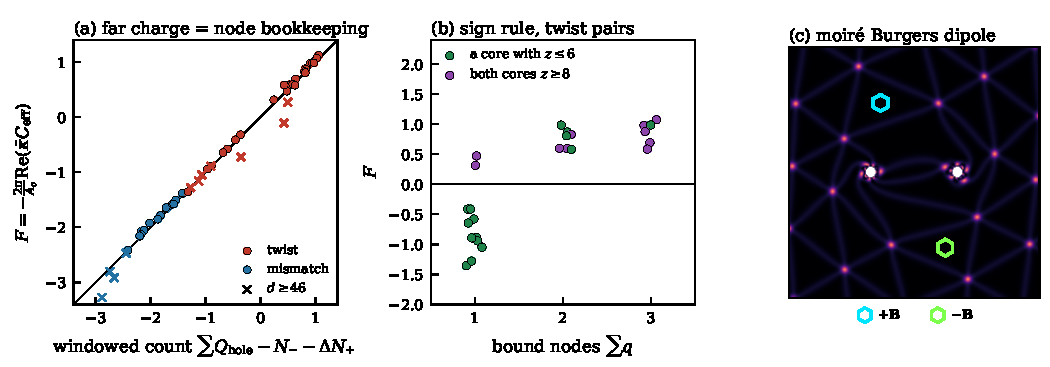
\includegraphics[width=\textwidth]{figs/fig6.pdf}
\caption{Integer bookkeeping.
(a) Far charge $F$ versus the window-weighted integer count of Eq.~\eqref{eq:bookkeeping} for 53 pair states (crosses: $d\ge46$, cores close to the window edge).
(b) Sign rule for twisted pairs ($16\le d\le46$): $F$ versus the total bound charge $\sum q$, colored by the smallest core valence.
(c) Geometric moir\'e Burgers circuits in a pulled twisted pair ($d=40$): hexagons mark Delaunay triangles of nodes with a non-closing circuit; their $\pm B$ form a dipole.}
\label{fig:book}
\end{figure*}

%=====================================================================
\section{Moir\'e elasticity and the ring-traction identity}\label{sec:elastic}
%=====================================================================

\subsection{Elastic constants of the moir\'e crystal}

We define the Eulerian moir\'e displacement $U$ by $u=\kappa(z-U)$ and impose homogeneous strains $U=U_az+U_b\bar z$ on oblique periodic cells spanned by the strained moir\'e vectors ($2\times2$ moir\'e cells). We then fit the relaxed energy density as
\begin{equation}
e=e_0+\sigma_d\varepsilon_d+2K_M\varepsilon_d^2+\tfrac12\chi_M\omega^2+2\mu_M|\gamma|^2+\dots,
\label{eq:moduli}
\end{equation}
with $\varepsilon_d={\rm Re}\,U_a$, $\omega={\rm Im}\,U_a$ and $\gamma=U_b$ (35 strain states, residual $<10^{-8}\theta^2$). All terms forbidden by hexagonal symmetry---linear shear, anisotropy, and the $\varepsilon_d\omega$ cross term---vanish within numerical precision. The results (Table~\ref{tab:moduli}, Fig.~\ref{fig:moduli}) differ qualitatively from the unrelaxed values. A moir\'e dilation is an atomic rotation in the twisted case and an atomic dilation in the mismatch case, which fixes the bare entries.

\begin{table}[t]
\caption{Moir\'e elastic constants in units of $\theta^2$ ($\lambda=-0.5$, $\mu=1$). The last row gives the values without registry relaxation (twist/mismatch).}
\label{tab:moduli}
\begin{ruledtabular}
\begin{tabular}{lccccc}
 & $K_M$ & $\mu_M$ & $\chi_M$ & $\sigma_d$ & $K_M/(K_M+\mu_M)$\\
\hline
twist & $-0.149$ & $1.149$ & $6.41$ & $-3.34$ & $-0.149$\\
mismatch & $0.273$ & $0.479$ & $-1.29$ & $-5.92$ & $0.363$\\
bare & $0/0.5$ & $1/1$ & $2/0$ & -- & $0/0.33$\\
\end{tabular}
\end{ruledtabular}
\end{table}

Two signs stand out. The twisted moir\'e has a \emph{negative bulk modulus}: a uniform moir\'e dilation (a local untwisting) lowers the energy. It is stable only because the longitudinal modulus $K_M+\mu_M=1.000\,\theta^2$ remains positive; we note that this coincides with the unrelaxed value. The mismatch moir\'e has a \emph{negative rotational stiffness}: it tends to rotate spontaneously, which explains the global rotation observed in mismatch backgrounds. In clamped boxes the bulk moir\'e expands uniformly, $\varepsilon_0\approx\Delta^*/L$ with $\Delta^*\approx2.7$--$3.0$ for the twist [Fig.~\ref{fig:moduli}(c)]. The excess twist is stored in an edge layer near the clamp. Treating the bulk as uniform and the edge layer as a line energy $g(\Delta)$ of the mismatch $\Delta=(\varepsilon_b-\eta)L$, the equilibrium condition $g'(\Delta)=-\sigma_d/2-2K_M\varepsilon_b$ is dominated by $\sigma_d$. This explains the $1/L$ law. The edge is nevertheless stiff: when a dilation $\eta$ is imposed on the clamp, the bulk follows it almost one to one [Fig.~\ref{fig:moduli}(d)].

\begin{figure*}[t]
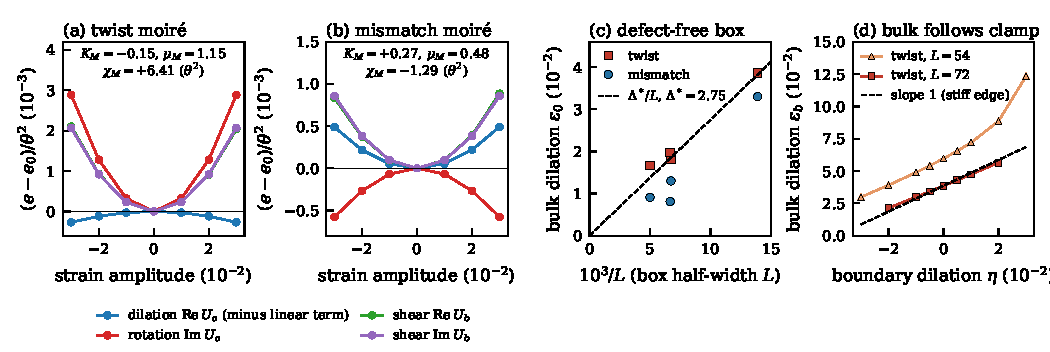
\includegraphics[width=\textwidth]{figs/fig7.pdf}
\caption{Elasticity of the moir\'e crystal.
(a),(b) Relaxed energy density versus homogeneous moir\'e strain for the twisted and mismatch moir\'e (periodic cells). The linear pre-stress term $\sigma_d\varepsilon_d$ has been subtracted from the dilation curve; the fitted constants are given in units of $\theta^2$.
(c) Uniform bulk dilation $\varepsilon_0$ of defect-free clamped boxes versus inverse box half-width.
(d) Bulk dilation of twisted boxes versus a dilation $\eta$ imposed on the clamped boundary; the dashed line has slope one.}
\label{fig:moduli}
\end{figure*}

\subsection{A local moir\'e source}

If these constants governed local sources, a disk of inserted moir\'e area $\delta A^*=2\pi r_0^2\varepsilon^*$ would send the fraction $S=K_M/(K_M+\mu_M)$ of it to infinity, in analogy with an Eshelby inclusion~\cite{Eshelby1957}. The far factor would then be $f=1-S$: 1.15 for the twist and 0.64 for the mismatch. To test this we construct the moir\'e analog of an eigenstrain inclusion. Inside a disk $D$ of radius $r_0$ centred at $z_0$, the energy is evaluated at $u+s$ instead of $u$, with $s=\varepsilon^*\kappa(z-z_0)\,\mathbb{1}_D$. The registry potential becomes $V(u+s)$ and $\varepsilon^*\kappa$ is added to the elastic gradient. The natural state inside is a moir\'e dilated by $\varepsilon^*$, and the jump of $s$ at $\partial D$ is a ring of fractional moir\'e dislocations.

The far response, measured from exact node positions, does not follow $S$. In twisted and mismatch moir\'es with $r_0=45$--$95$ (1.5--3.2 moir\'e periods) in boxes of half-width 150 and 200, $S=A/(\varepsilon^*r_0^2)$ ranges from $-8$ to $+5.5$. Here $A$ is the coefficient of the far field $A(1/r-r/L_{\rm eff}^2)$, whose effective radius $L_{\rm eff}$ always matches the box. The value of $S$ depends on $r_0$, on whether the ring passes through a node shell, and on the sign of $\varepsilon^*$ [Fig.~\ref{fig:ring}(d)].

\subsection{Ring-traction identity}

The reason is an exact identity. Let $u_0$ be the equilibrium at $\varepsilon^*=0$ and $w=\kappa(z-z_0)$. By the envelope theorem,
\begin{equation*}
E_1\equiv\frac{\partial E}{\partial\varepsilon^*}\Big|_0=\int_D\sigma_{\rm at}:\nabla w\,\dd A+\int_D\nabla V(u_0)\cdot w\,\dd A ,
\end{equation*}
where $\sigma_{\rm at}$ is the atomic Cauchy stress of $u_0$. The equilibrium condition $\nabla V(u_0)={\rm div}\,\sigma_{\rm at}$ and one integration by parts cancel the bulk terms exactly:
\begin{equation}
E_1=\oint_{\partial D}\big(\sigma_{\rm at}\,n\big)\cdot\kappa\,(z-z_0)\,\dd l .
\label{eq:ring}
\end{equation}
The local source therefore couples only to the microscopic traction on its boundary [Fig.~\ref{fig:ring}(a)]. For the twist, $\kappa(z-z_0)$ is tangential and $E_1=\theta r_0\oint t_t\,\dd l$ is the microscopic torque on the ring. Averaged over the position $z_0$ within a moir\'e cell, the mean stress is symmetric and $\langle E_1\rangle=0$. For the mismatch, $\kappa(z-z_0)$ is radial and $E_1=\theta r_0\oint t_n\,\dd l$. The mean atomic stress produced by the background strain $\theta$ gives $\langle E_1\rangle=4(\lambda+\mu)\theta^2\pi r_0^2$, which equals $2\theta^2\pi r_0^2$ here. A continuum moir\'e description would instead predict $E_1=-\pi r_0^2\sigma_d$ ($+57$ and $+101$ at $r_0=70$ for twist and mismatch). This coupling is absent.

Table~\ref{tab:ring} and Fig.~\ref{fig:ring}(b,c) verify Eq.~\eqref{eq:ring}. Evaluated on the baseline field alone, it reproduces the finite-difference drive of the inclusion runs within 1--2\% in the linear regime ($|\varepsilon^*|\le0.01$). Averages over 16 ring centres agree with the predicted means within one standard error. The fluctuation between placements grows in proportion to $r_0$. For $r_0\lesssim3$ moir\'e periods it is as large as the mean, and the centred, sixfold-symmetric ring is always an extreme. The negative-$\varepsilon^*$ jumps seen in the mismatch runs are rearrangements of nodes next to the ring, where the drive is concentrated.

\begin{table}[b]
\caption{Ring-traction identity, Eq.~\eqref{eq:ring}. $E_1$ from the ring integral on the baseline field, from finite differences of the inclusion runs, and the mean $\pm$ standard deviation over 16 ring centres, compared with the predicted mean.}
\label{tab:ring}
\begin{ruledtabular}
\begin{tabular}{lccccc}
 & $r_0$ (box) & identity & runs & 16 centres & pred.\\
\hline
twist & 45 (150) & $-8.82$ & $-8.80$ & $-0.4\pm2.9$ & 0\\
twist & 70 (150) & $-16.94$ & $-16.84$ & $-1.7\pm9.0$ & 0\\
mism. & 45 (150) & $0.88$ & $0.90$ & $14.1\pm4.2$ & 14.1\\
mism. & 60 (150) & $33.10$ & $32.6$ & $26.5\pm7.4$ & 25.1\\
mism. & 70 (150) & $7.65$ & $7.76$ & $32.2\pm11.2$ & 34.2\\
mism. & 95 (200) & $21.99$ & -- & $60.8\pm21.2$ & 63.0\\
\end{tabular}
\end{ruledtabular}
\end{table}

\begin{figure*}[t]
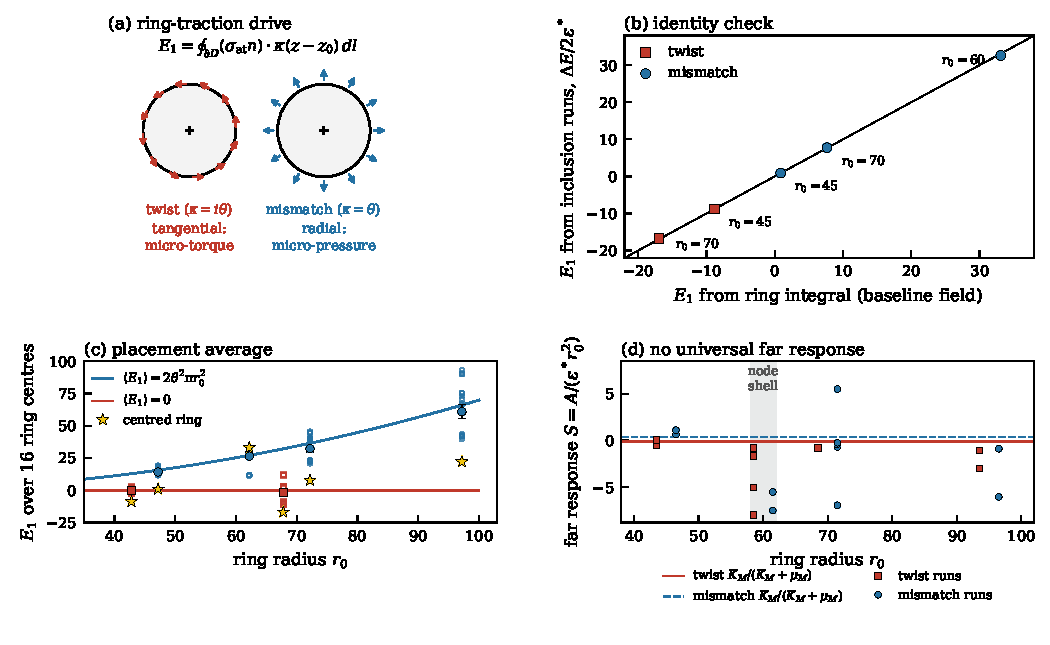
\includegraphics[width=\textwidth]{figs/fig8.pdf}
\caption{Ring-traction identity.
(a) The drive of a local moir\'e source is the atomic traction integrated against $\kappa(z-z_0)$ on its boundary: tangential (micro-torque) for the twist, radial (micro-pressure) for the mismatch.
(b) $E_1$ from Eq.~\eqref{eq:ring} on the baseline field versus the finite-difference drive of the inclusion runs.
(c) $E_1$ for 16 ring centres per radius (small symbols), their mean $\pm$ standard error, and the centred ring (stars), compared with the predicted means $0$ (twist) and $2\theta^2\pi r_0^2$ (mismatch).
(d) Far response $S=A/(\varepsilon^*r_0^2)$ of all inclusion runs. No common value emerges, in particular not the Eshelby value $K_M/(K_M+\mu_M)$ (horizontal lines). The gray band marks a ring lying on a node shell.}
\label{fig:ring}
\end{figure*}

\subsection{Consequence}

The same argument applies to every moir\'e-scale defect embedded in a continuous registry, including the geometric $\pm B$ dipoles of Fig.~\ref{fig:book}(c). Such defects couple to the atomic layer through the forces their cores exert, not through the coarse-grained moir\'e constants. Consequently, \emph{the far node charge of a defect configuration is fully described by integer bookkeeping [Eq.~\eqref{eq:bookkeeping}] together with the force-dipole dressing [Eq.~\eqref{eq:dipole}].} No universal coefficient $f$ converts an inserted moir\'e area into far charge. The moir\'e constants of Table~\ref{tab:moduli} describe homogeneous strains, such as the boundary-driven and $1/L$ bulk dilations of Fig.~\ref{fig:moduli}.

%=====================================================================
\section{Discussion}\label{sec:disc}
%=====================================================================

\emph{Hierarchy of charges.} The affine map $u=\kappa U$ relates atomic and moir\'e defects level by level (Table~\ref{tab:hier}). Disclinations and dislocations are homotopy invariants ($\pi_1(T^2)=\mathbb{Z}^2$ and the point group). Because $A$ maps lattice to lattice, an integer atomic invariant becomes an integer moir\'e invariant. The atomic area charge is quantized by the number of atoms but is not a homotopy invariant ($\pi_2(T^2)=0$), whereas the moir\'e node number is a degree. The continuous parameter $\theta$ sits in between, so the far share $\theta n_{\rm miss}\cos\varphi_m$ is fractional, and the integer local share of the nonlinear core makes up the difference. Writing the node density as the Jacobian $(1/4\pi^2)\epsilon^{ab}\partial_a\phi_1\partial_b\phi_2$ of the two moir\'e phases $\phi_i=\bm G_i\cdot u$ makes the analogy with Goldstone--Wilczek induced charge explicit~\cite{Goldstone1981}.

\begin{table}[t]
\caption{Defect hierarchy under $u=\kappa U$.}
\label{tab:hier}
\begin{ruledtabular}\small
\begin{tabular}{lccc}
level & atomic & moir\'e & in own units\\
\hline
disclination & $s\in60^\circ\mathbb{Z}$ & same $s$ & integer\\
dislocation & $b\in\Lambda$ & $B=A^{-1}b\in\Lambda_M$ & integer\\
area/torque & $C$ (complex) & $m=C/\kappa$ & $\times\theta$ (fractional)\\
\end{tabular}
\end{ruledtabular}
\end{table}

\emph{Twist versus mismatch.} The two backgrounds differ only in $\alpha$, but the consequences are distinct. (i) Area defects are swallowed with $b_s=\sqrt2R$ in a twisted moir\'e and not at all in a mismatch moir\'e. Frustrated integer assignment in the twisted case produces multiple branches and hysteresis. (ii) Relaxation of the twisted moir\'e is rotational and its walls are shear walls, so the bulk modulus drops out of the defect problem. Mismatch relaxation is dilational and sensitive to $K$. (iii) The mismatch background is mirror symmetric, so node rotation is an Ising-like variable; this is consistent with $\chi_M<0$ and with the spontaneous chirality at large $K$. In the twisted background the mirror is absent and node rotation is pinned.

\emph{Experimental consequences.} The counting rule $T=\theta n_{\rm miss}$ predicts that in twisted bilayer graphene at $\theta\approx1.1^\circ$ a vacancy cluster in one layer missing about $1/\theta\approx52$ unit cells ($\approx100$ atoms, $\approx2.7$~nm$^2$) removes one moir\'e node. The Einstein radius is then $R=\sqrt{|C|/\theta}\approx4.8$~nm for a moir\'e period of $12.8$~nm. For an area defect in a twisted bilayer the node is bound to the defect and swallowed within $\sqrt2R\approx7$~nm. For a mismatch heterostructure such as graphene on hBN (mismatch $\approx1.8\%$), the same defect leaves the local pattern intact and spreads the node deficit to the boundary as a smooth distortion. Both regimes can be imaged by scanning tunneling microscopy, piezoresponse, or interferometric moir\'e metrology~\cite{Kerelsky2019,Uri2020,Halbertal2021,Kazmierczak2021}, around irradiation-induced vacancy clusters~\cite{Banhart2011}. Our results also imply that the moir\'e distortion around such defects carries information about integer branches, i.e., the core state. Two defects with the same atomic content can differ in far node charge by up to $\sim3$ nodes.

\emph{Model assumptions.} The topological statements (Secs.~\ref{sec:topo} and~\ref{sec:lens}A) hold for any continuous registry map with vanishing Burgers class. The partition theorem relies on the linear region outside the core, i.e., on $R$ being larger than the wall width. It also requires that the registry forces produce no net stress on average over the moir\'e lattice. For realistic vacancy clusters of tens of atoms at $\theta$ of order one degree, both conditions are met. The single-field description neglects layer-resolved displacement and out-of-plane relaxation; these change $V$ and the elastic constants but not the topology or the lens structure. The numerical branch search is not exhaustive, and the nudged-elastic-band barriers~\cite{Henkelman2000} we computed for branch switching are upper bounds.

%=====================================================================
\section{Conclusions}\label{sec:concl}
%=====================================================================

Moir\'e nodes are topological charges of the registry map, and atomic area defects act on them as gravitational lenses with mass $m=C/\kappa$. A defect missing $n_{\rm miss}$ unit cells removes $\theta n_{\rm miss}$ ordinary nodes. A fraction $1-\cos\varphi_m$ is swallowed and bound to the core as an integer, and a fraction $\cos\varphi_m$ is pushed to infinity. This explains why area defects are swallowed in twisted bilayers but not in mismatch heterostructures, and why closing and opening irises are symmetric in one case and not in the other. Beyond the atomic charge, the far node charge is dressed by the force dipole of the reorganized registry forces. This induced charge depends on the integer branch the pattern selects and behaves as a displacement-controlled source. The moir\'e crystal has its own anomalous elastic constants---a negative bulk modulus for twist and a negative rotational stiffness for mismatch. Yet local sources couple to the microscopic ring traction rather than to these constants, so no universal moir\'e response coefficient exists. Integer bookkeeping plus force-dipole dressing is the complete description of the far field. Open problems include an integer-resolved version of the partition theorem, a rule that predicts $C_{\rm reg}$ from the core state, and the node currents pumped by moving defects.

\begin{acknowledgments}
% Funding information to be added by the author.
Numerical calculations and parts of the analysis and drafting were carried out with the assistance of an AI model (Claude, Anthropic); the author takes full responsibility for the content.
\end{acknowledgments}

\section*{Data availability}
Code and analysis data are available at \url{https://github.com/cywon-commits/moire-iris-lens}.

\appendix

\section{Equivalence of elastic references}\label{app:ref}
The clamped calculations assign elastic energy to the strain of the total $u$, i.e., $E_{\rm el}[u]=E_{\rm el}[u_b]+E_{\rm el}[\delta u]+\int\sigma_b:\varepsilon(\delta u)$. For affine $u_b$ the stress $\sigma_b$ is uniform, and the cross term becomes the boundary integral $\oint\sigma_bn\cdot\delta u$. It vanishes on the outer boundary ($\delta u=0$). On a core rim $\sigma_b$ is isotropic (mismatch) or zero (twist), so the cross term couples only to the mean normal displacement, which is fixed by the constraint. The cross term is therefore a constant, and equilibria, energy differences and interactions agree between the two references.

\section{Removed node charge of a pair}\label{app:pair}
For two defects, $J=1-|f'|^2$ with $f'=-m_1/(\bar z-\bar z_1)^2-m_2/(\bar z-\bar z_2)^2$. Averaged over translations, the number of removed ordinary nodes is $n_M\int(1-J\,\mathbb{1}_{J>0})\dd^2z=n_M\int\min(1,|f'|^2)\dd^2z$. For one defect this gives $2\pi R^2n_M=T$, consistent with Eq.~\eqref{eq:partition}. Numerically, $(+,+)$ pairs give $1.79$--$1.93$, and $(+,-)$ pairs give $0.02,0.93,1.46,1.90$ at $d=0,8,16,30$.

\section{Counting}\label{app:count}
\emph{Nodes:} on each grid cell, we count the windings of the polygon formed by the registry values at its four corners around the AA lattice points. Shared edges cancel, so Eq.~\eqref{eq:gauss} holds exactly on the grid. \emph{$Q_{\rm hole}$:} winding along a staircase loop just outside the core (radius $\approx3$). \emph{$z$:} changes of the AB/BA label along circles of radius 5, 7 and 9. \emph{Node positions} for the inclusion analysis are obtained by solving $u(z)=c_{\rm AA}+n$ with Newton iterations on a cubic interpolant (residual $<10^{-12}$).

\section{Numerical parameters}\label{app:num}
\begin{table}[h]
\caption{Parameters (lattice constant $a=1$).}
\label{tab:param}
\begin{ruledtabular}\small
\begin{tabular}{ll}
twist angle or mismatch $\theta$ & $1/30$\\
registry $V_0$, $V_3$ & $0.005$, $\sqrt3V_0$\\
Lam\'e $\mu$; $\lambda$ & $1$; $-0.5$ or $1$\\
 $K/\mu=(\lambda+\mu)/\mu$ & $0.5$ or $2$\\
$|C|$, core radius $r_h$, rim penalty & $4$, $2.4$, $200$\\
Einstein radius $R=\sqrt{|C|/\theta}$ & $\approx11$\\
grid spacing $h$ & $0.45$\\
box half-width & 72; 109.8, 148.5, 150, 200\\
relaxed moir\'e period & $\approx31$\\
\end{tabular}
\end{ruledtabular}
\end{table}

\begin{thebibliography}{99}

\bibitem{Bistritzer2011} R. Bistritzer and A. H. MacDonald, Moir\'e bands in twisted double-layer graphene, \href{https://doi.org/10.1073/pnas.1108174108}{Proc. Natl. Acad. Sci. USA \textbf{108}, 12233 (2011)}.

\bibitem{Cao2018a} Y. Cao, V. Fatemi, S. Fang, K. Watanabe, T. Taniguchi, E. Kaxiras, and P. Jarillo-Herrero, Unconventional superconductivity in magic-angle graphene superlattices, \href{https://doi.org/10.1038/nature26160}{Nature \textbf{556}, 43 (2018)}.

\bibitem{Cao2018b} Y. Cao \emph{et al.}, Correlated insulator behaviour at half-filling in magic-angle graphene superlattices, \href{https://doi.org/10.1038/nature26154}{Nature \textbf{556}, 80 (2018)}.

\bibitem{Andrei2020} E. Y. Andrei and A. H. MacDonald, Graphene bilayers with a twist, \href{https://doi.org/10.1038/s41563-020-00840-0}{Nat. Mater. \textbf{19}, 1265 (2020)}.

\bibitem{Kennes2021} D. M. Kennes \emph{et al.}, Moir\'e heterostructures as a condensed-matter quantum simulator, \href{https://doi.org/10.1038/s41567-020-01154-3}{Nat. Phys. \textbf{17}, 155 (2021)}.

\bibitem{Popov2011} A. M. Popov, I. V. Lebedeva, A. A. Knizhnik, Yu. E. Lozovik, and B. V. Potapkin, Commensurate-incommensurate phase transition in bilayer graphene, \href{https://doi.org/10.1103/PhysRevB.84.045404}{Phys. Rev. B \textbf{84}, 045404 (2011)}.

\bibitem{Alden2013} J. S. Alden \emph{et al.}, Strain solitons and topological defects in bilayer graphene, \href{https://doi.org/10.1073/pnas.1309394110}{Proc. Natl. Acad. Sci. USA \textbf{110}, 11256 (2013)}.

\bibitem{Nam2017} N. N. T. Nam and M. Koshino, Lattice relaxation and energy band modulation in twisted bilayer graphene, \href{https://doi.org/10.1103/PhysRevB.96.075311}{Phys. Rev. B \textbf{96}, 075311 (2017)}.

\bibitem{Carr2018} S. Carr, D. Massatt, S. B. Torrisi, P. Cazeaux, M. Luskin, and E. Kaxiras, Relaxation and domain formation in incommensurate two-dimensional heterostructures, \href{https://doi.org/10.1103/PhysRevB.98.224102}{Phys. Rev. B \textbf{98}, 224102 (2018)}.

\bibitem{Yoo2019} H. Yoo \emph{et al.}, Atomic and electronic reconstruction at the van der Waals interface in twisted bilayer graphene, \href{https://doi.org/10.1038/s41563-019-0346-z}{Nat. Mater. \textbf{18}, 448 (2019)}.

\bibitem{Dai2016} S. Dai, Y. Xiang, and D. J. Srolovitz, Twisted bilayer graphene: Moir\'e with a twist, \href{https://doi.org/10.1021/acs.nanolett.6b02870}{Nano Lett. \textbf{16}, 5923 (2016)}.

\bibitem{Gargiulo2018} F. Gargiulo and O. V. Yazyev, Structural and electronic transformation in low-angle twisted bilayer graphene, \href{https://doi.org/10.1088/2053-1583/aa9640}{2D Mater. \textbf{5}, 015019 (2018)}.

\bibitem{Zhang2018} K. Zhang and E. B. Tadmor, Structural and electron diffraction scaling of twisted graphene bilayers, \href{https://doi.org/10.1016/j.jmps.2017.12.005}{J. Mech. Phys. Solids \textbf{112}, 225 (2018)}.

\bibitem{Uri2020} A. Uri \emph{et al.}, Mapping the twist-angle disorder and Landau levels in magic-angle graphene, \href{https://doi.org/10.1038/s41586-020-2255-3}{Nature \textbf{581}, 47 (2020)}.

\bibitem{Kerelsky2019} A. Kerelsky \emph{et al.}, Maximized electron interactions at the magic angle in twisted bilayer graphene, \href{https://doi.org/10.1038/s41586-019-1431-9}{Nature \textbf{572}, 95 (2019)}.

\bibitem{Huder2018} L. Huder, A. Artaud, T. Le Quang, G. Trambly de Laissardi\`ere, A. G. M. Jansen, G. Lapertot, C. Chapelier, and V. T. Renard, Electronic spectrum of twisted graphene layers under heterostrain, \href{https://doi.org/10.1103/PhysRevLett.120.156405}{Phys. Rev. Lett. \textbf{120}, 156405 (2018)}.

\bibitem{Kazmierczak2021} N. P. Kazmierczak \emph{et al.}, Strain fields in twisted bilayer graphene, \href{https://doi.org/10.1038/s41563-021-00973-w}{Nat. Mater. \textbf{20}, 956 (2021)}.

\bibitem{Halbertal2021} D. Halbertal \emph{et al.}, Moir\'e metrology of energy landscapes in van der Waals heterostructures, \href{https://doi.org/10.1038/s41467-020-20428-1}{Nat. Commun. \textbf{12}, 242 (2021)}.

\bibitem{Lau2022} C. N. Lau, M. W. Bockrath, K. F. Mak, and F. Zhang, Reproducibility in the fabrication and physics of moir\'e materials, \href{https://doi.org/10.1038/s41586-021-04173-z}{Nature \textbf{602}, 41 (2022)}.

\bibitem{Banhart2011} F. Banhart, J. Kotakoski, and A. V. Krasheninnikov, Structural defects in graphene, \href{https://doi.org/10.1021/nn102598m}{ACS Nano \textbf{5}, 26 (2011)}.

\bibitem{Einstein1936} A. Einstein, Lens-like action of a star by the deviation of light in the gravitational field, \href{https://doi.org/10.1126/science.84.2188.506}{Science \textbf{84}, 506 (1936)}.

\bibitem{Schneider1992} P. Schneider, J. Ehlers, and E. E. Falco, \emph{Gravitational Lenses} (Springer, Berlin, 1992).

\bibitem{Nelson2002} D. R. Nelson, \emph{Defects and Geometry in Condensed Matter Physics} (Cambridge University Press, Cambridge, 2002).

\bibitem{Kleman2008} M. Kl\'eman and J. Friedel, Disclinations, dislocations, and continuous defects: A reappraisal, \href{https://doi.org/10.1103/RevModPhys.80.61}{Rev. Mod. Phys. \textbf{80}, 61 (2008)}.

\bibitem{Mermin1979} N. D. Mermin, The topological theory of defects in ordered media, \href{https://doi.org/10.1103/RevModPhys.51.591}{Rev. Mod. Phys. \textbf{51}, 591 (1979)}.

\bibitem{Eshelby1957} J. D. Eshelby, The determination of the elastic field of an ellipsoidal inclusion, and related problems, \href{https://doi.org/10.1098/rspa.1957.0133}{Proc. R. Soc. London A \textbf{241}, 376 (1957)}.

\bibitem{Landau1986} L. D. Landau and E. M. Lifshitz, \emph{Theory of Elasticity}, 3rd ed. (Pergamon, Oxford, 1986).

\bibitem{Goldstone1981} J. Goldstone and F. Wilczek, Fractional quantum numbers on solitons, \href{https://doi.org/10.1103/PhysRevLett.47.986}{Phys. Rev. Lett. \textbf{47}, 986 (1981)}.

\bibitem{Liu1989} D. C. Liu and J. Nocedal, On the limited memory BFGS method for large scale optimization, \href{https://doi.org/10.1007/BF01589116}{Math. Program. \textbf{45}, 503 (1989)}.

\bibitem{Henkelman2000} G. Henkelman, B. P. Uberuaga, and H. J\'onsson, A climbing image nudged elastic band method for finding saddle points and minimum energy paths, \href{https://doi.org/10.1063/1.1329672}{J. Chem. Phys. \textbf{113}, 9901 (2000)}.

\end{thebibliography}

\end{document}
